% !TeX spellcheck = en_GB
%%%%%%%%%%%%%%%%%%%%%%%%%% phdsymp_sample2e.tex %%%%%%%%%%%%%%%%%%%%%%%%%%%%%%
%% changes for phdsymp.cls marked with !PN
%% except all occ. of phdsymp.sty changed phdsymp.cls
%%%%%%%%%%              %%%%%%%%%%%%%
%%%%%%%%%% More information: see the header of phdsymp.cls %%%%%%%%%%%%%
%%%%%%%%%%              %%%%%%%%%%%%%
%%%%%%%%%%%%%%%%%%%%%%%%%%%%%%%%%%%%%%%%%%%%%%%%%%%%%%%%%%%%%%%%%%%%%%%%%%%%%%%


\documentclass[twocolumn]{phdsymp} %!PN

\usepackage[english]{babel}  % Voor nederlandstalige hyphenatie (woordsplitsing)

\usepackage{graphicx}     % Om figuren te kunnen verwerken
\usepackage{graphics}			% Om figuren te verwerken.

\graphicspath{images/}

\PassOptionsToPackage{hyphens}{url}
\usepackage{url}

\usepackage[T1]{fontenc}

\usepackage{amsmath}
\usepackage{packages/customcommands}

\hyphenation{}

\def\BibTeX{{\rm B\kern-.05em{\sc i\kern-.025em b}\kern-.08em
 T\kern-.1667em\lower.7ex\hbox{E}\kern-.125emX}}

\newtheorem{theorem}{Theorem}

\begin{document}

\title{Client-side evaluation of GeoSPARQL queries over heterogeneous data sources} %!PN

\author{Andreas De Witte}

\supervisor{dr. ing. Pieter Colpaert, dr. ir. Ruben Taelman, Brecht Van de Vyvere, Julian Andres Rojas Melendez}

\maketitle

\begin{abstract}
    On the Web as it's currently known, users can easily understand pages of websites. This is not the case for computers, as they need to do a lot of effort to substract both meaning and context from sentences. The Web, as it is today, is not built to be interpreted by machines. Thanks to the Semantic Web, which is an extension to the current Web, it is possible for machines to understand the pages of websites.

    It is currently possible to query for linked data to a limited amount of data sources, because very few data sources support linked data. These data sources can be heterogeneous, which means they can be different types of data sources. Theses queries are executed with SPARQL, which has multiple working implementations. For geographical queries, GeoSPARQL is needed. However, there are only few implementations of GeoSPARQL and most of these implementations are working incorrectly.

    In this work, a limited implementation of GeoSPARQL is made in order to request data in RDF format and calculate the topological relations in this data. With this implementation, it has been tested for which interfaces these topological relations can be calculated on the client-side. Doing this on the client-side is important for many reasons. The major reason is that many of these calculations would cripple a server, while these calculations for only one user on the client-side is very possible. In other words, doing this on the client-side is an effective way of spreading the load. This paper gives new insights about handling geographical queries on the client-side.

    Like this, it seems to be very simple to calculate the topological relations on the client-side when the data source is a data dump. Hereby, the client wil have to download the entire data set. It's also possible to calculate topological relations when the source is a TPF interface. The interface will already provide several optimizations by only returning the necessary data. However, when the source is a SPARQL endpoint, this is more difficult. This is possible by iterating over the different RDF triples and by counting the amount of matching results. Like this, the smallest pattern can be formed and retrieved from the SPARQL endpoint. This prevents the retrieval of unnecessary data.
    
    The conclusion can be made that these kind of queries can be handled better on the client-side. Like this, the entire query can be processed, even when the source doesn't fully support it. This master's thesis is mostly useful for computer scientists who are true experts about Semantic Web, but it can also be used by enthousiasts who want to receive a better understanding of the Semantic Web and it's possibilities.
\end{abstract}

\begin{keywords}
    Semantic Web, linked data, OGC, Geo-SPARQL, client-side, topological relation
\end{keywords}

\section{Introduction}
The Web is made to be understood by humans. However, this makes it harder for machines to interprete the Web. Because of this, simple tasks are very hard to automate. An example of this is planning a daytrip. The idea with this would be that an intelligent agent would be fully capable of autonomously planning the daytrip, keeping in mind the participants, the weather, common interests,\dots

The Web has some other flaws too. For example, bigger companies (like Google, Facebook,\dots) are collecting huge amounts of data about people, while this should rather be managed by the people themselves. Like this, the person himself would be able to decide which data he wants to share and more importantly, which data he doesn't want to share. This would be possible using Linked Data, which is discussed later on.

This extension to the Web is called the Semantic Web. This Web uses Linked Data, which is queried using SPARQL (a query language). GeoSPARQL is an extension of SPARQL. This as well will be discussed more broadly, later on.

This article focusses on the extension of the different ``Linked Data publcation'' interfaces. Hereby, the goal is to extend these interfaces with GeoSPARQL functionalities by executing the filtering on the client.

\section{State of the art}
The Semantic Web is a Web that can be interpreted by both humans and machines. To make the Semantic Web a reality, several steps are needed. Hereby, meaning is important for computers. Also, this has to be represented in a way machines can understand, which is done with RDF (= Resource Description Framework). Both these problems are tackled with Linked Data. Another important aspect of the Semantic Web is decentralization. This means that there can not be a single entity that holds all the data, but instead many small entities that each hold a little part of the data \cite{berners2001semantic}. 

Apart from posting data on the Web, the Semantic Web has another (and even more important) goal, being the creation of links. When data is retrieved, this data should contain links to where related data can be found. By doing so, the data gets more context. It's important that this data is both open and accessible to be reused \cite{berners2001semantic}.

RDF provides a general method to describe relations between data objects. This makes RDF most efficient to integrate information from multiple sources, by decoupling the information from it's scheme. RDF uses triples, which have the form ``subject - predicate - object'' \cite{lassila1998resource}. It is important to know that RDF is not a data format, but a data model. This means that the data must be serialized before it can be published. The most used RDF syntaxes are: ``RDF/XML'', ``RDFa'', ``Turtle'', ``N-Triples'' and ``JSON-LD''. In these formats, ``Turtle'' is the most compact one and ``JSON-LD'' is the most used one (because of it's similarities with the well known JSON format) \cite{heath2011linked}.

SPARQL is a query language of querying RDF based data. This language has many similarities with SQL. SPARQL is actually a query language, used for retrieving data from the Web. The importance of SPARQL for this master's thesis is that a GeoSPARQL implementation requires a working SPARQL implementation, because GeoSPARQL is an extension of SPARQL \cite{sparql2013querylanguage}.

Comunica is a modular SPARQL query engine for the Web, made by the IDLAB of the university of Ghent. Comunica is the working implementation of SPARQL that is used as a start. Hereby, Comunica is chosen because it was developed with five specific goals \cite{taelman2018comunica}:
\begin{enumerate}
    \item It must be able to evaluate SPARQL queries; 
    \item It must be modular;
    \item It must be able to query over heterogeneous interfaces;
    \item It must be able of querying federated (= multiple sources at once);
    \item It must be made using web technologies.
\end{enumerate}

The OGC (= Open Geospatial Consortium) is a worldwide community that tries to improve the way that geospatial location information is handled. To achieve its goal, the OGC provides standards like ``GML'' and ``WKT'' for the description of geographical objects. As well, GeoSPARQL is an OGC standard \cite{ogcdocs}.

GeoSPARQL is one of the many OGC standards and is mostly fit for the execution of GIS (= geographical Information System) queries. However, this is not its only possibility. GeoSPARQL uses RDF and is an extension on SPARQL. It brings a new vocabulary for representing geospatial data. To do so, it uses an architecture (see \figurerefEN{fig:abstr_geosparql_architecture}) which contains one main class, being ``SpatialObject''. The other two classes, ``Feature'' and ``Geometry'', are both inherited from the ``SpatialObject'' class.  It's important to know that a ``Feature'' object must contain a ``Geometry'' object. A ``Geometry'' is represented by a ``GML literal'' or a ``WKT literal'' \cite{ogcdocs}.

\begin{figure}[ht]
    \centering
    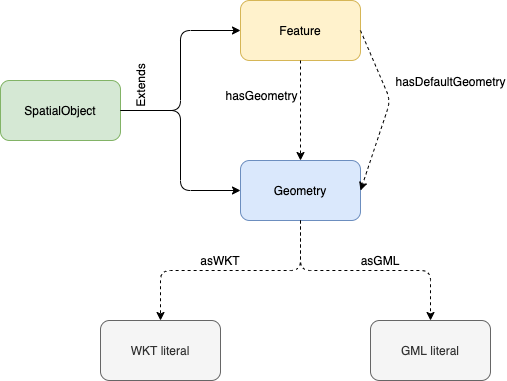
\includegraphics[width=\linewidth]{images/geosparql_architecture.png}
    \caption{Simplified diagram of the GeoSPARQL classes ``Feature'' and ``Geometry'' with some properties (figure based on \protect\cite{geosparqlsupport}).}
    \label{fig:abstr_geosparql_architecture}
\end{figure}

With GeoSPARQL, it's important to distinguish the topological functions from the non-topological functions. Topological functions describe relations between objects (for example whether an object lies inside another object or not), while non-topologiscal functions are more varied (for example returning the distance between two objects).

\begin{figure}[ht]
    \centering
    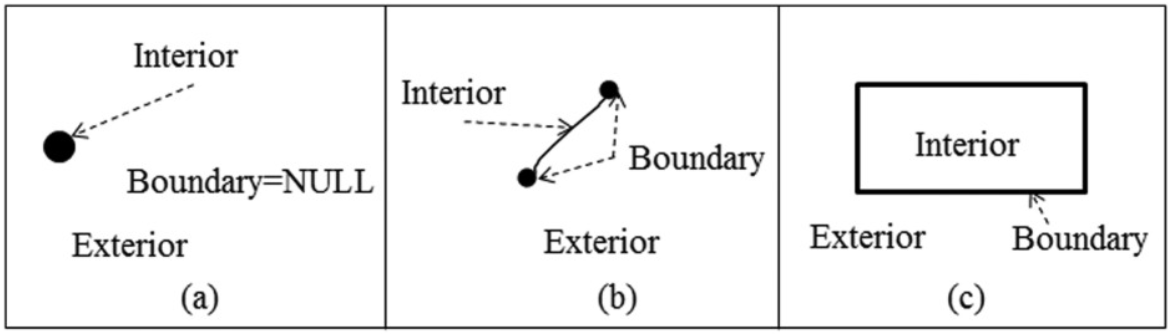
\includegraphics[width=\linewidth]{images/spatial_objects_DE-9IM.png}
    \caption{Spatial objects with their interior, boundary and exterior: (a) A point; (b) A Line; (c) A polygon. Figure from \protect\cite{shen2018classification}}.
    \label{fig:abstr_de-9im}
\end{figure}

In order to describe topological relation using Geo-SPARQL, the DE-9IM (= Dimensionally Extended Nine-Intersection) model is used. This model is a 3x3 matrix that compares the interior, boundary and exterior of two spatial objects. The meaning of interior, boundary and exterior are clarified in \figurerefEN{fig:abstr_de-9im}. The 3x3 matrix for two objects ``a'' and ``b'' has the following form \cite{shen2018classification}:

\begin{equation*}
    DE-9IM(a,b) = 
\end{equation*}
\begin{equation*}
    \begin{bmatrix}
        dim(I(a)\cap I(b)) & dim(I(a)\cap B(b)) & dim(I(a)\cap E(b))\\
        dim(B(a)\cap I(b)) & dim(B(a)\cap B(b)) & dim(B(a)\cap E(b))\\
        dim(E(a)\cap I(b)) & dim(E(a)\cap B(b)) & dim(E(a)\cap E(b))
    \end{bmatrix}
\end{equation*}

Last but not least, GeoSPARQL brings a functionality to rewrite a query. this is needed when a topological function is used as a predicate. This is needed because this can only exist as a predicate when this has been pre computed on the server. This is not mentioned again in this master's thesis since the filtering is done on the client, hence assumptions of pre computations on the server can not be made. Another argument to not assume pre computations on the server is that data can originate from multiple sources. This means it's not useful to pre compute this on the server \cite{ogcdocs}.

\section{Implementation}
Comunica is used for the implementation of the GeoSPARQL functionalities. In Comunica, an actor is created who initializes a GeoSPARQL query engine. This actor uses ``sparqlalgebrajs'' in order to transform the SPARQL query into SPARQL algebra. Moreover, ``sparqlee'' is used to have a correct execution of the SPARQL algebra. In other words, ``sparqlee'' is an expression evaluator. With this implementation, the GeoSPARQL functionalities are implemented withing ``sparqlee''. 

To respect the datastructure of GeoSPARQL (see \figurerefEN{fig:abstr_geosparql_architecture}), GeoJSON is used. This is a format that's already widely used and supports both ``Geometry'' and ``Feature'' objects. In order to turn the ``WKT literal'' into GeoJSON, Terraformer is used.

The next problem that needs to be solved, is executing both topological functions and non-topological function. For this, ``Turf.js'' is used. Turf provides many methods that can be used to do calculations with geospatial objects. Besides, Turf has some built in functions (like ``booleanContains'') that are immediately usable. In addition to its funtional strength, Turf is a good choice because of its huge community. This community makes sure bugs are detected as fast as possible. Also, Turf is developed modularly, so only the small modules that are needed, have to be loaded.

The last thing to do to achieve a working implementation of GeoSPARQL is solve the problem of the different projections. This is solved thanks to ``Proj4js''. Proj4 is a library that takes care of the transformation from coordinates in one reference system to coordinates in another reference system.

Now, a working implementation of GeoSPARQL is available. Only one last implementation remains. This is a test environment to check which ``Linked Data publication'' interfaces can be extended with GeoSPARQL functionalities. To solve this, Comunica's ``jQuery Widget'' is used. This widget provides a graphical interface which enables the possibility to edit both the query and the sources used to execute the query. This graphical interface will also visualize the result of the query and it will show logging. This logging is mostly interesting to test this master's thesis. Thanks to the logging, it's possible to check how the program works internally. 
 
\section{Interfaces}
Before the different interfaces can be tested, an appropriate use-case is needed. Because of it being well known, Belgium has been chosen as use-case for the tests. Hereby, a shallow drawing of Belgium has been made, which is visualized in \figurerefEN{fig:abstr_demoset}. This drawing is made in a custom scale. Furthermore, this drawing is identical (in terms of coordinates) to the data set, which can be found on GitHub Gist\footnote{https://gist.github.com/dreeki/e48bbe533a4b1191045b3652ff2c9c81}. This data set is split into five different files (being: ``land'', ``gewest'', ``provincie'', ``weg'' and ``stad''. This respectively means ``country'', ``region'', ``province'', ``road'' and ``city'') in order to verify that federated querying is still possible.

\begin{figure}
    \centering
    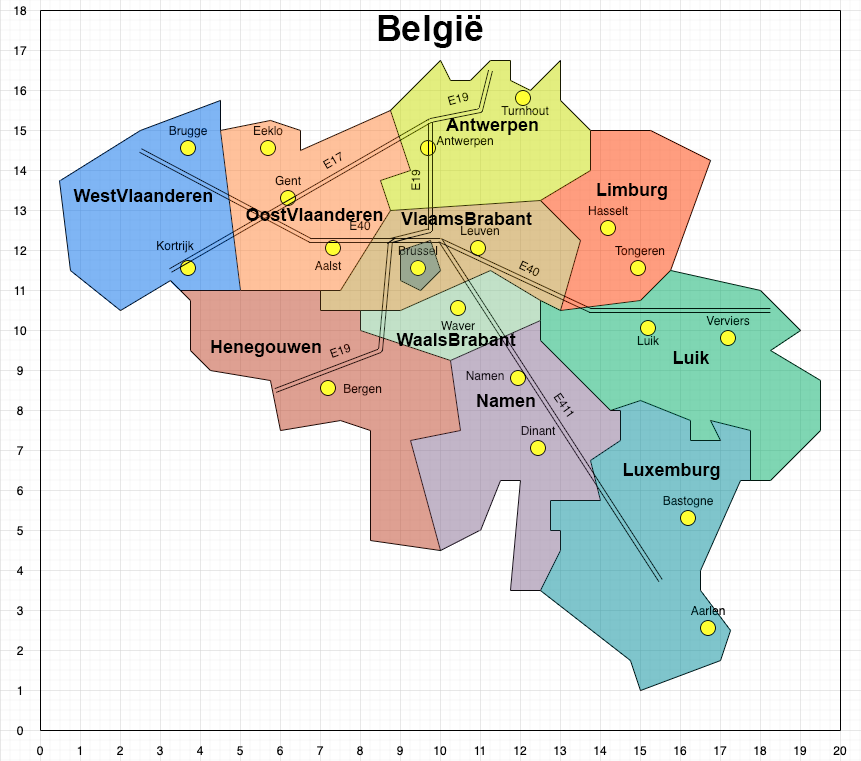
\includegraphics[width=\linewidth]{images/geosparql_demo.png}
    \caption{Test set to test different sources.}
    \label{fig:abstr_demoset}
\end{figure}

The first kind of source that has to be checked is the ``data dump''. This will also be used as a baseline because this is the easiest source. With the ``data dump'', the entirety of the data set is downloaded onto the client. By doing so, the client can fully execute the filtering.

The second kind of source is the ``TPF interface''. Hereby, the server will manage the files with data and respond to requests. While querying, the query itself will be divided into multiple triple pattern fragments, so the server itself can decide not to send overflowing information. Afterwards, the client will join these results so he can filter the total result in the end. Like this, the correct result can be retrieved.

The third and final source is the ``SPARQL endpoint''. This one is surely the hardest. This source has the possibility of executing SPARQL queries on its own, but it doesn't support GeoSPARQL. This means that it's impossible to send the GeoSPARQL query as a whole to the ``SPARQL endpoint'' (moreover, federated querying would be impossible if the ``SPARQL endpoint'' were to fully execute the query on its own). This problem is tackled by iterating over the query its individual RDF triples. Like this, the query engine will first send a ``count'' query in order to know what the smallest pattern is. This is needed to achieve a good performance. The second step is the actual retrieval of this smallest pattern. This is repeated multiple times, until the entire query is processed. In the end, the entirety of results is joined on the client, so the client is capable of executing the filtering once again.

\section{Conclusie}
To formulate an answer to the question which ``Linked Data publcation'' interfaces can be extended with GeoSPARQL functionalities by filtering on the client, the earlier results have to be interpreted.

This is possible for ``data dumps'' because the client downloads the entire data set and filters afterwards. For ``TPF interfaces'', this is also possible by joining the different triple pattern fragments on the client. The result can be filtered like this once again. Even with ``SPARQL endpoints'', it is possible by counting at the source how many results there are for each RDF triple in the query. Hereby, the smallest patterns are retrieved and joined on the client. This result is also filtered on the client.


\bibliographystyle{phdsymp}
%%%%%\bibliography{bib-file} % commented if *.bbl file included, as
%%%%%see below


%%%%%%%%%%%%%%%%% BIBLIOGRAPHY IN THE LaTeX file !!!!! %%%%%%%%%%%%%%%%%%%%%%%%
%% This is nothing else than the phdsymp_sample2e.bbl file that you would%%
%% obtain with BibTeX: you do not need to send around the *.bbl file  
%%
%%---------------------------------------------------------------------------%%
%
\begin{thebibliography}{1}
    \bibitem{berners2001semantic}
    Berners-Lee, Tim and Hendler, James and Lassila, Ora
    \newblock {\em The semantic web},
    \newblock Scientific american, vol. 284, no. 5, pp. 34–43, 2001.

    \bibitem{berners2006linkeddata}
    Berners Lee, Tim
    \newblock {\em Linked Data},
    \newblock 2006.

    \bibitem{lassila1998resource}
    Lassila, Ora and Swick, Ralph R and others
    \newblock {\em Resource description framework (RDF) model and syntax specification},
    \newblock 1998.

    \bibitem{heath2011linked}
    Heath, Tom and Bizer, Christian
    \newblock {\em Linked data: Evolving the web into a global data space},
    \newblock Synthesis lectures on the semantic web: theory and technology, vol. 1, no. 1, pp. 1–136, 2011.

    \bibitem{sparql2013querylanguage}
    Harris, Steve and Seaborne, Andy
    \newblock {\em SPARQL 1.1 Query Language},
    \newblock World Wide Web Consortium, 2013.

    \bibitem{taelman2018comunica}
    Taelman, Ruben and Van Herwegen, Joachim and Vander Sande, Miel and Verborgh, Ruben
    \newblock {\em Comunica: a modular SPARQL query engine for the web},
    \newblock in International Semantic Web Conference. Springer, 2018, pp. 239–255.

    \bibitem{ogcdocs}
    \newblock {\em Open Geospatial Consortium},
    \newblock URL: https://ogc.org

    \bibitem{geosparqlsupport}
    \newblock {\em GeoSPARQL support: What is GeoSPARQL},
    \newblock URL: http://graphdb.ontotext.com/documentation/standard/geosparql-support.html

    \bibitem{shen2018classification}
    Shen, Jingwei and Chen, Min and Liu, Xintao
    \newblock {\em Classification of topological relations between spatial objects in two-dimensional space within the dimensionally extended 9-intersection model},
    \newblock Transactions in GIS, vol. 22, no. 2, pp. 514–541, 2018.
\end{thebibliography}
%
%%---------------------------------------------------------------------------%%


\end{document}